\chapter{Umsetzung}
Im Rahmen dieser Arbeit entstand ein in C++ geschriebenes Programm welches den Marching Cubes Algorithmus auf eine Voxelmenge anwendet und das Resultat via OpgenGL visualisiert. Des Weiteren ist es möglich das verarbeitete Model als STereoLithography (.stl) Datei zu exportieren.
\section{Marching Cubes}
Der Marching Cubes Algorithmus ist das Herzstück der entstandenen Applikation er ermöglicht die Umrechnung der gegebenen Voxel Datenmenge in eine polygonale Darstellung welche sich im später vergleichsweise einfach darstellen lässt.
\subsection{Allgemein}
Die Implementierung ist eine angepasst Version der von [ref] bereitgestellten Umsetzung. Die wesentlichen Änderungen sind die Auslagerung der Funktionen in eine eigenen Klasse und das verwenden anderer Datenstrukturen. Durch die Umstellung auf STL-Behälter und der daraus folgende Verzicht auf C-Strukturen welche zur Laufzeit immer neuen Speicher anfordern konnte die Geschwindigkeit enorm erhöht werde.
\subsection{Klasse}
\begin{figure}[H]
	\centering
	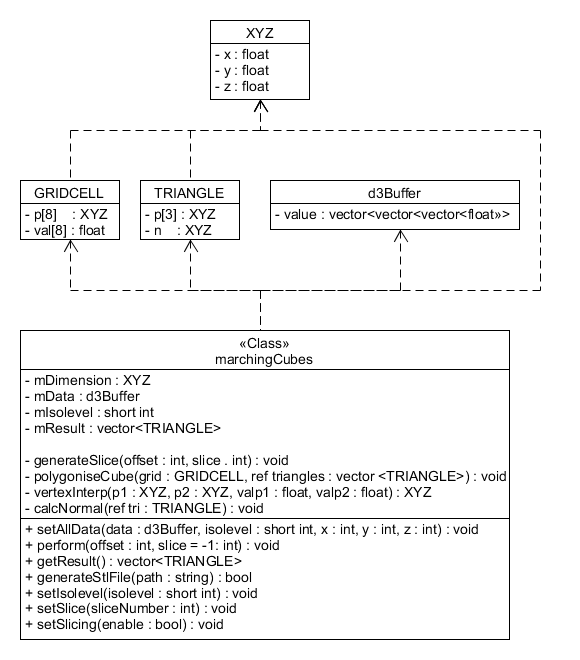
\includegraphics[width=.90\textwidth]{marchingCubes}
	\caption{UML-Diagramm der marchingCubes Klasse}
	\label{fig:marchingCubes}
\end{figure}
\subsection{Auszüge Implementierung}

\section{File Formate}

\subsection{Allgemein}
\subsection{Image File (.img)}

\subsection{Header File (.hdr)}

\subsection{STereoLithography (.stl)}
\ref{prog:generateSTL}
\subsection{Klasse}
\begin{figure}[H]
	\centering
	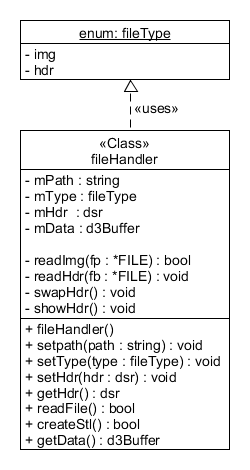
\includegraphics[width=.60\textwidth]{fileHandler}
	\caption{UML-Diagramm der fileHandler Klasse}
	\label{fig:fileHandler}
\end{figure}
\begin{program}
	\caption{Generierung einer STL-Datei}
	\label{prog:generateSTL}
	\begin{CCode}
	bool marchingCubes::GenerateStlFile(std::string path){
		FILE *fptr = NULL;
		fprintf(stderr, "Writing triangles ...\n");
		if ((fptr = fopen(path.c_str(), "a+b")) == NULL) {
			fprintf(stderr, "Failed to open output file\n");
			return false;
		}
		char fileHeader[81] = "solid Test Head";
		char bytes[3] = { 0x00, 0x00 };
		fwrite(&fileHeader, sizeof(fileHeader)-1, 1, fptr);
		fwrite(&ntri, sizeof(int), 1, fptr);
		for (int i = 0; i < ntri; i++) {
			fwrite(&tri[i].n[0], sizeof(float), 3, fptr);
			for (int k = 0; k < 3; k++)  {
				fwrite(&tri[i].p[k], sizeof(float), 3, fptr);
			}
			fwrite(bytes, 2, 1, fptr);
		}
		fclose(fptr);
		return true;
	}
	\end{CCode}
\end{program}

\section{OpenGL}
\subsection{Allgmein}
\subsection{Schnittstelle (Klasse)}
\subsection{Klasse}
\begin{figure}[H]
	\centering
	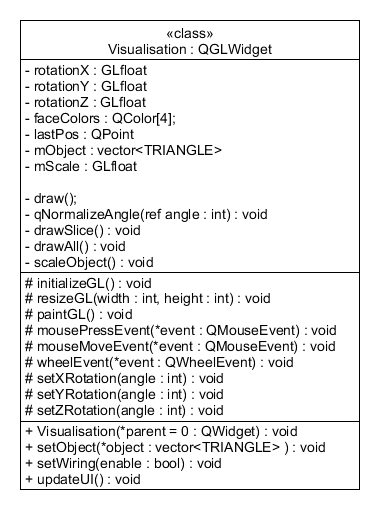
\includegraphics[width=.70\textwidth]{visualisation}
	\caption{UML-Diagramm der Visualisation Klasse}
	\label{fig:visualisation}
\end{figure}

\subsection{Auszüge Implementierung}
\begin{program}
	\caption{Berechnung der Normalen eines Dreiecks}
	\label{prog:calcNormal}
\begin{CCode}
	void marchingCubes::CalcNormal(TRIANGLE &tri){
		XYZ U;
		XYZ V;
		U.x = tri.p[1].x - tri.p[0].x;
		U.y = tri.p[1].y - tri.p[0].y;
		U.z = tri.p[1].z - tri.p[0].z;
		
		V.x = tri.p[2].x - tri.p[0].x;
		V.y = tri.p[2].y - tri.p[0].y;
		V.z = tri.p[2].z - tri.p[0].z;
		
		tri.n[0].x = (U.y * V.z) - (U.z * V.y);
		tri.n[0].y = (U.z * V.x) - (U.x * V.z);
		tri.n[0].z = (U.x * V.y) - (U.y * V.x);
	}
\end{CCode}
\end{program}

\section{Benutzeroberfläche}